% Authorship: Claude-drafted, author-revised
\section{The Threshold Governs How Much Law}

The second of Part VI's two questions is whether the divergence among the
mechanisms is an artifact of the determinacy threshold. Stated that way it
invites a second defense, and a defense is arguably the wrong shape for this
parameter. The threshold is the parameter Berman expressly declines to fix. It is not the only quantity this
Article chooses rather than reads off his text. The correlation structure of
the activations is equally a modeling choice, and Section VIII.B finds it
carries more of the substantive results than the threshold does. Unlike
the correlation structure, the threshold is a choice Berman addresses and
leaves open. He writes
that an aggregative system ``could incorporate thresholds or eschew
them,'' commits to neither, and has pressed the point
directly.\footnote{Berman, \textit{Practices}, \textit{supra} note 7, at
331 (an aggregative system ``could incorporate thresholds or eschew
them''). In correspondence he confirmed that his claim is that some
threshold is available to such a system, not that one is required.
E-mail from Mitchell N.\ Berman to author (Mar.\ 2026) (on file with
author). Nothing here rests on the correspondence; the published text is
sufficient and the correspondence confirms it. That the faithful baseline
is accordingly the bare sign of net force, $\tau = 0$, is \textit{supra}
Part~III.A; see also \textit{supra} Part~IV.A.}

The quantity itself is easy to state. Net force is the signed number the
weighted sum returns, positive for one side of the case and negative for
the other, and a case counts as determinate when the size of that number
exceeds $\tau$. Below $\tau$ the model reports the case as unresolved
rather than deciding it by a hair. At $\tau = 0$ nothing is withheld and the bare sign decides everything. At
$\tau = 0.2$, the value used throughout this Article, about one case in
seven comes back unresolved. As a modeling decision, Parts III and IV both
flagged that value and deferred it here.

So the threshold is the Article's rather than Berman's, and a parameter
the theory declines to fix calls for a statement of scope rather than a
defense: the results reported so far that it governs, set against the
results it does not. The answer would seem to divide cleanly. On the evidence below, the threshold governs how much of the law comes out
determinate, and it governs that almost completely. It does not appear to
govern the model's substantive properties, which turn on the
structure of the cases rather than on where the line is drawn. Everything
in this Part, the answer to Part VI's second question included, would seem
to follow from that division.

This Part takes Berman's concession at full strength and reports that
the model cannot repair it, since nothing internal to the model selects a
positive threshold. It then measures what the threshold does control,
returns to the one comparison Part VII had to decline, and states how much
is left standing for the second finding.

\subsection{A Choice the Theory Does Not Make}

On this Berman's published text leaves the threshold open, and asked about
it he confirmed that his claim is that some threshold is available to an
aggregative system, not that one is required. In Part III the consequence
is recorded: the faithful baseline is the bare sign of net force, and a
positive $\tau$ is a confidence gate this Article imposes for reasons of
its own. Nothing about the concession is grudging. It is correct, and the rest of
this Section is what the model says once it is taken seriously. Whether
some future version of the theory would want a threshold is a question the
model cannot reach.

For every mechanism tested, sweep $\tau$ upward from zero and the share of
cases decided falls smoothly and monotonically. It begins at
$D(0) = 1.000$, the value deciding by the bare sign amounts to:
exact equipoise has probability zero on continuously distributed
activations, so at $\tau = 0$ every case has a verdict. From there the
curve descends without a kink, a plateau, or an interior optimum,
reaching between $0.794$ and $0.828$ at $\tau = 0.30$ depending on the
mechanism. This is not a feature of the draws. On independent activations the determinacy
rate has a closed form in $\tau$, proved as Theorem 4 in Part IV and verified
again here on a finer grid running down to $\tau = 0$, which the simulation
matches to a maximum error of $0.0106$. The form is a Gaussian tail in
the ratio of the threshold to the dispersion of net force, and that
dispersion is $\sigma_F = 1.141$ on the weight vector used
throughout.\footnote{The closed form is
$D(\tau) = 2\left(1 - \Phi(\tau/\sigma_F)\right)$, where $\Phi$ is the
standard normal distribution function and $\sigma_F^2 = \frac{1}{3}\sum_i
w_i^2$ is the variance of net force; here $\sigma_F = 1.141$. This is Theorem~4, \textit{supra} Part~IV.D. Part~IV reports a maximum
error of $0.006$ over the coarser grid used there, which starts at $\tau =
0.05$; verified again on the finer grid of this Part, which runs down to
$\tau = 0$, the residual is $0.0106$ over $\tau \in [0, 0.40]$. The theorem is not degrading, the grid is denser and reaches further toward
the origin. Both residuals measure the quality of the normal approximation the
closed form rests on rather than the fidelity of the implementation. The form
is derived for independently drawn activations and does not carry over to
correlated ones, which is why the threshold sweeps of this Part are conducted
on independent draws. The global sensitivity analysis of Section VIII.B is
not; it varies the activation correlation deliberately and so tests something
else. The formula is separable in the threshold and the weights, which meet
only through the ratio $\tau/\sigma_F$, and Section~VIII.B is consistent with
that separability
independently: the threshold's interactions with the other three inputs carry $0.028$ of the
variance. That decomposition runs over a design sweeping the activation
correlation from zero to $0.9$, so it spans the region where the margin over
the hierarchical Hart reverses sign, which Part IV reports at $-0.054$ under
category correlation. What it shows is that the threshold does not govern
whether that requirement holds. The activation structure does.}


A parameter with a privileged value would have something on its response
curve to point at: an elbow where the returns change, a saturation point, a
discontinuity where the model's behavior changes character. This curve
has none of that. Between $\tau = 0$ and $\tau = 0.30$ it loses about
seven points of determinacy for every $0.10$ of threshold and does
nothing else. On the curve's own evidence any value in that range would seem as
defensible as any other, and the default of $0.20$, at which the stipulated
engine decides $86.2\%$ of cases, is a convention rather than a discovery. Figure~\ref{fig:f3-threshold} shows the curve for the
stipulated engine and for the three mechanisms the sweep rebuilds.

\begin{figure}[t]
\centering
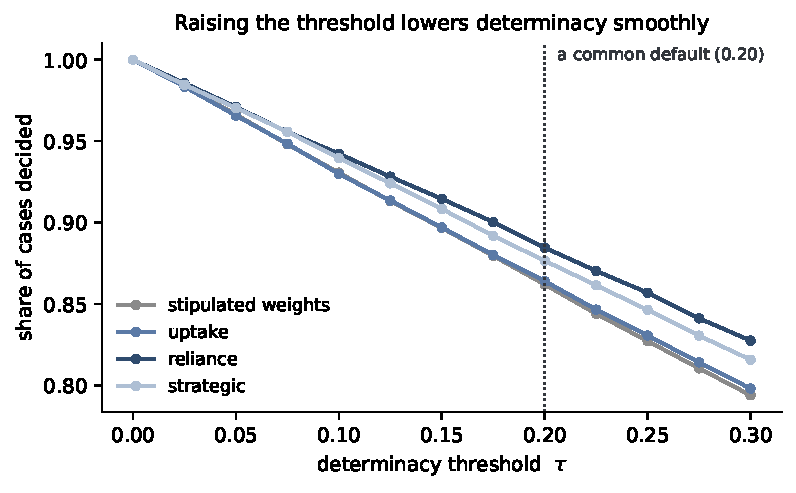
\includegraphics[width=\textwidth]{F3_threshold_choice}
\caption{The determinacy threshold is a choice the theory does not make.
A case counts as determinate when the size of its net force exceeds the
threshold $\tau$. Raising $\tau$ lowers the share of cases decided
smoothly and monotonically for every mechanism, from $1.000$ at
$\tau = 0$ to between $0.794$ and $0.828$ at $\tau = 0.30$, with no kink,
no plateau, and no privileged value anywhere on the curve; $0.20$ is a
common default and is marked for reference. The curve has a closed form
in $\tau$, which the simulation matches to a maximum error of $0.0106$.
Berman's text permits an aggregative system to eschew thresholds
altogether, so the faithful baseline is the bare sign of net force, the
$\tau = 0$ end of this figure, where determinacy is at its maximum.
Curves are thirty-seed means for the stipulated engine of Part~IV and for
the uptake, reliance, and strategic mechanisms of Part~VI; the
appointment mechanism's weights come from a separate simulation this
sweep does not rebuild. All four requirements of Part~III hold across the
whole range for each of the three emergent mechanisms plotted.}
\label{fig:f3-threshold}
\end{figure}

A reader may reasonably ask whether some criterion outside the curve
picks a value. Two are available, and they do not agree. A per-case
robustness criterion asks which verdicts survive perturbation of the
weights and sets the band to discard exactly the cases a small error
would flip; across thirty seeds it recommends $\tau^{*} = 0.267$ (standard deviation
$0.010$). A cumulative criterion asks instead at what $\tau$ nine in ten of
the still-determinate verdicts are robust. It recommends $0.075$ (standard
deviation $0.008$), and that figure is probably biased low, since it averages the fragile cases near the margin in with
the safe interior. The two are not two ends of one interval. They answer different questions and land three and a half times apart, so
neither can plausibly be read as fixing the other, and the conventional
$0.20$ sits between them, below the per-case value and above
the cumulative floor.\footnote{The per-case criterion perturbs the
weights with Gaussian noise of standard deviation $0.10$, calls a verdict
robust when its direction survives in at least ninety percent of draws,
and takes the smallest net force at and above which verdicts are reliably
robust: $\tau^{*} = 0.267$ (sd $0.010$) across thirty seeds. The
cumulative criterion asks instead at what $\tau$ ninety percent of all
still-determinate verdicts are robust, and returns $0.075$ (sd $0.008$).
The per-case value scales with the assumed noise, $\tau^{*} \approx 2.67$
standard deviations of it, and moves with both undefended choices: across
assumed noise of $0.05$, $0.10$, and $0.15$ crossed with confidence
levels of ninety-five and ninety percent, it runs from $0.137$ to
$0.495$, with the conventional $0.20$ above the recommendation in two of
those six cells and below it in four (eight-seed means).}

Neither derivation is unconditional, which is the sharper point. Rather than a constant, the per-case value is a multiple of the assumed
weight noise, $2.67$ standard deviations of it. So it moves with both the
noise scale and the confidence level one assumes, running from $0.137$ to
$0.495$ across the plausible grid. The robustness analysis fixes a
confidence level and a noise scale. It does not fix a number.

The last resort would be to let the model choose. It cannot, and for a
structural reason rather than a computational one. Because determinacy is
monotone decreasing in $\tau$, the determinacy-maximizing threshold is
exactly zero, and there is no interior optimum for any procedure aimed at
deciding more cases to find. Every positive threshold is bought by
declining to decide cases the model could decide. That is a defensible
purchase if activation is evidence relative and a court should not treat
a hair's-breadth balance as settling a question, but it is a purchase
made on grounds outside the model.\footnote{$D(\tau)$ is monotone
decreasing for every mechanism tested: for the stipulated engine
$D(0) = 1.000$, $D(0.20) = 0.862$, $D(0.255) = 0.832$. A procedure
selecting the threshold by maximizing how much law the model declares
determinate would therefore return the bare-sign rule, which is Berman's
own baseline and not a positive threshold at all. A procedure that
instead lets the model calibrate the threshold against its own verdicts
returns a value with no variance across seeds, the signature of a
self-referential fixed point rather than of an optimum.}

The theory does not fix the threshold and the model does not fix it
either. It is a choice, and this Article makes it at $0.20$ for
convention rather than for cause. After that, the Article owes not a
justification of the number but an account of its work.

\subsection{How Much, Not Whether}

A parameter the theory leaves blank is a liability in proportion to what
it controls, so the question is what varies when the threshold varies.
Here the instrument is a global sensitivity analysis, which apportions the
variance in an output among four inputs varied together: the threshold,
the dispersion of the weights, the correlation among the principles'
activations, and the share of principles carrying no weight at all, called
sparsity below.
Unlike moving one knob at a time from a fixed starting point, this
measures each input's contribution across the whole space rather than at
one location in it.\footnote{First-order and total-order variance shares
are Sobol indices on a Saltelli design of $8{,}192$ base samples, with
total-order indices by the Jansen estimator and $95\%$ intervals from
$2{,}000$ bootstrap resamples; the implementation reproduces the analytic
indices of the Ishigami benchmark to a maximum error of $0.0002$. The
inputs vary over: threshold $[0.05, 0.30]$, weight dispersion
$[0, 0.30]$, activation correlation $[0, 0.9]$, and share of principles
zeroed, from none to four of nine. The threshold range starts at $0.05$,
so the bare-sign baseline is not inside this variance budget. Each
evaluation runs the same fixed stream of $8{,}000$ cases, so a difference
in output can come only from the four inputs. For a dominant input the
first-order estimate is noisy, its interval running from $0.462$ to
$1.210$, so the tight total-order index of $0.849$ (interval $0.827$ to
$0.871$) rather than the first-order estimate of $0.822$ is the reliable
measure of dominance. The first-order shares sum to about $0.96$, so the
model is nearly additive here.}

On the determinacy rate the threshold dominates, and the point is
conceded without qualification. Across the four inputs varied together, its
total-order share of the variance is $0.849$, with a $95\%$ confidence
interval from $0.827$ to $0.871$. Activation correlation is a distant second at
$0.156$, sparsity third at $0.023$, and weight dispersion effectively
nothing at $0.008$. As far as it goes, the sharpest form of the worry is therefore correct: how
much law this model declares determinate is very nearly a function of where
the line is drawn. Every determinacy figure in this Article should be read
with that in mind.

Run the identical decomposition, with the threshold threaded through in
the same way, on the two substantive outputs, and the ordering reverses.
On the margin over the hierarchical Hart the threshold's first-order
share falls to $0.176$ while activation correlation rises to $0.810$. On
the magnitude probe the reversal is wider still, $0.020$ against $0.919$.
On this evidence the threshold's grip would appear to be specific rather
than general. It reaches how much law comes out determinate. It does not
reach how the decisions look once made.
Figure~\ref{fig:f4-sensitivity} sets the two decompositions side by side.

\begin{figure}[t]
\centering
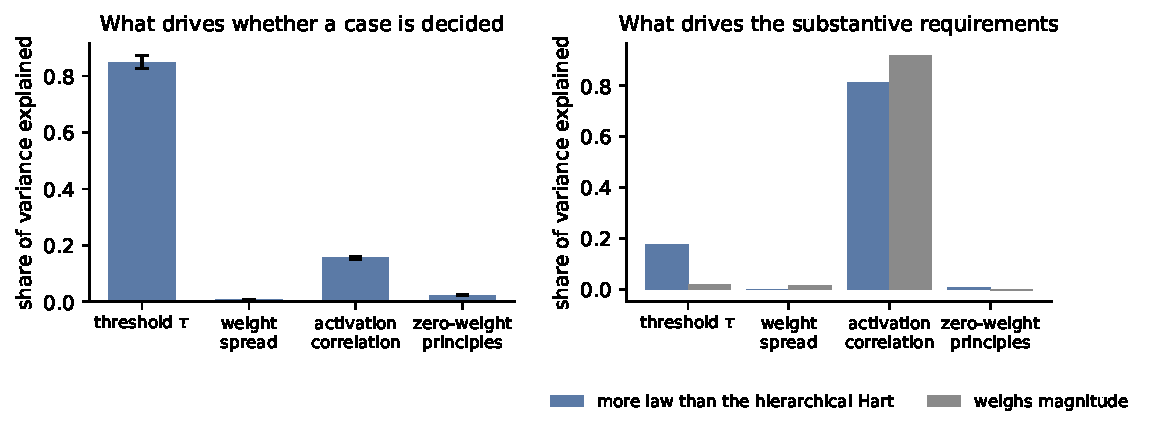
\includegraphics[width=\textwidth]{F4_sensitivity}
\caption{What the threshold governs. A global sensitivity analysis
apportions the variance in each output among four inputs varied together:
the threshold, the weights' dispersion, the correlation among
activations, and the share of principles carrying no weight.
\textit{Left}: for whether a case is decided at all, the
threshold dominates, taking a total-order variance share of $0.849$
($95\%$ confidence interval $0.827$ to $0.871$), against $0.156$ for
activation correlation, $0.023$ for sparsity, and $0.008$ for weight
dispersion. \textit{Right}: for the substantive requirements the ordering
reverses. On the margin over the hierarchical Hart the threshold's
first-order share is $0.176$ against activation correlation's $0.810$,
and on the magnitude probe $0.020$ against $0.919$. The left panel
reports total-order shares, which include each input's interactions with
the others; the right panel reports first-order shares from a smaller run
and should be read as a ranking rather than as precise shares. On that
smaller run the threshold takes $0.635$ of the determinacy variance
against activation correlation's $0.267$, so the reversal holds within a
single design. The threshold governs how much law comes out determinate.
It does not govern whether the model's substantive properties hold.}
\label{fig:f4-sensitivity}
\end{figure}

Before anything is drawn from it, the comparison has to be made
like-for-like, and the reversal is measured inside a single panel rather
than across two runs. In that panel the threshold's first-order share of the
determinacy variance is $0.635$ against correlation's $0.267$, so the
ordering flips between outputs measured the same way on the same design.
Two limits travel with it. The sample is small, so the figures should be read as a ranking rather than
as precise shares. And the magnitude probe varies so
little across this space that its decomposition is only weakly
informative, which leaves the Hart-margin panel to carry the
point.\footnote{The comparison across outputs uses a smaller design of
$256$ base samples and $1{,}500$ cases per evaluation, since only the
ordering is at issue. First-order shares, by input and output: determinacy
rate, threshold $0.635$ and activation correlation $0.267$; margin over
the hierarchical Hart, $0.176$ and $0.810$; magnitude probe, $0.020$ and
$0.919$. The left panel of Figure~\ref{fig:f4-sensitivity} reports
total-order shares from the large design and the right panel first-order
shares from this one, so $0.849$ and $0.176$ are not two measurements of
the same kind; the within-panel figures just given are. Activation
correlation moves the correlation and the scale of the activations
together, and weight dispersion and sparsity both act on weight
magnitudes, so the smaller shares are best read jointly rather than as
cleanly separate effects.}

The reversal has a cause, and naming it turns a report into an
explanation. Deciding a case at its highest-ranked applicable tier, the hierarchical
Hart of Part IV consults no threshold at all, so its determinacy rate
does not move with $\tau$ while the weighted sum's does.
Raising the threshold therefore displaces the margin between them by
exactly the amount it displaces determinacy: over $\tau$ from $0$ to
$0.30$ the determinacy rate falls by $0.206$ and the margin over the
hierarchical Hart falls by $0.206$. The threshold would seem to shift the margin without shaping it. What shapes it is the correlation structure of the
cases, moving the weighted sum and the Hart baseline by different
amounts and so fixing how large the displaced quantity is in the first
place.\footnote{Within a fixed activation regime the margin is the
determinacy rate less a constant, since the hierarchical Hart's rate is
invariant to $\tau$: across $\tau$ from $0$ to $0.30$ both fall by
$0.206$, from $1.000$ to $0.794$ and from $+0.407$ to $+0.201$
respectively. Across the sensitivity sweep the baseline is not constant,
because activation correlation moves the Hart rate as well as the
weighted sum's, which is why correlation takes the larger share of the
margin's variance while the threshold merely displaces it.}

Across this Article's claims, the threshold sets the volume of law and
almost nothing else. The weighted sum's margin over the hierarchical Hart,
and its sensitivity to magnitude rather than rank, turn on how the cases are
structured. A reader who thinks the threshold was chosen badly is
entitled to a different determinacy rate. That reader is not thereby
entitled to a different answer on any of the four requirements, and the last Section of this Part reports what happens when the threshold
is swept across its whole defensible range.

\subsection{The Gated and the Ungated}

Part VII declined one comparison and said why it had to. Except the gated weighted sum, every rule in its battery is ungated, so
each converts every case into a verdict and posts a determinacy rate of
$1.000$.
Against the hierarchical Hart's $59.4\%$ on that battery the ungated
rules show an apparent margin of $+0.406$ where the gated weighted sum
shows $+0.268$. Part VII named the inflation a threshold artifact and
handed the diagnosis here.

The diagnosis is that $+0.406$ is a point on this Part's curve. Nothing
about it is a property of ordinal aggregation or of lexical priority. It
is the margin over the hierarchical Hart at $\tau = 0$. Read
off the threshold sweep run here, on the stipulated engine and a
different battery of cases, the margin runs from $+0.407$ at $\tau = 0$
through $+0.269$ at $\tau = 0.2$ to $+0.201$ at $\tau = 0.30$. The
ungated rules' apparent fourteen-point advantage is the distance between
two points on that curve, and two runs sharing no cases reproduce the
$\tau = 0$ value to within a thousandth.\footnote{\textit{Supra}
Part~VII.B. The hierarchical Hart decides $59.4\%$ of that battery, so
the ungated rules' determinacy of $1.000$ yields an apparent margin of
$1.000 - 0.594 = +0.406$ against the gated weighted sum's $+0.268$ at
$\tau = 0.2$. This Part's sweep, on the stipulated engine over a
different battery and thirty seeds, puts the margin at $+0.407$ at
$\tau = 0$, $+0.269$ at $\tau = 0.2$, and $+0.201$ at $\tau = 0.30$. Two
independent runs reproducing the same figure to a thousandth is what
identifies $+0.406$ as the $\tau = 0$ point on a curve rather than as a
property of any rule.}

Where the artifact lands makes this a correction rather than a defense. On the faithful members of the cardinal family it falls exactly as it falls
on the lexical foils, and it falls hardest on the rule Berman himself endorses.
Because exact equipoise has probability zero, the bare-sign rule of Part
III never abstains, so it posts a perfect determinacy rate and the full
$+0.406$ margin for no substantive reason whatever. Berman's
own baseline is the most inflated rule in the battery.

The general rule this yields is probably what a later reader needs. A determinacy
rate and a margin over the hierarchical Hart are properties of a rule and
a threshold together, never of a rule alone. Any figure of either kind
reported in this Article carries a threshold with it, and comparing two
such figures across rules gated differently compares the gates. The
remedy is not to prefer one setting over another. It is to state the
setting alongside the number, as this Article does, and to
note that the closed form given above converts any such figure to any other threshold
directly.

\subsection{What the Threshold Leaves Standing}

Rebuilding the emergent weights once per seed and sweeping only the
evaluation threshold, from $\tau = 0$ to $\tau = 0.30$ in steps of
$0.025$ over thirty seeds, the four requirements of Part III continue to
hold at every threshold for each of the three emergent mechanisms the
sweep rebuilds, including at Berman's own $\tau = 0$. The requirement
that comes closest to its criterion does so at that baseline, for a
reason Part VII supplies: the magnitude probe scores lower on an ungated
rule than on a gated one, $0.0229$ against $0.0496$, because a gated rule
can also be pushed across the determinacy threshold by a magnitude-only
change, so the five-fold bar is hardest to clear at $\tau = 0$, where the
strategic mechanism clears it on exactly nine seeds in ten. On determinacy the mechanism ordering is invariant as well, reliance above
strategic above uptake, at every threshold above zero; at $\tau = 0$ the ordering is
a degenerate tie, since every mechanism decides essentially every
case.\footnote{The emergent weights are built once per seed, which is the
expensive step, and only the evaluation threshold sweeps, so the
comparison is like-for-like across $\tau$; thirty seeds, $\tau$ from $0$
to $0.30$ in steps of $0.025$, $800$ cases per seed. The requirements are
scored per seed as in Part~III and counted as holding at a threshold when
at least nine seeds in ten pass; the determinacy ordering is invariant for
every $\tau \geq 0.025$. The appointment mechanism's weights come from a
separate simulation this sweep does not rebuild, so it is not carried
through the threshold grid; its noise tolerance is the narrowest of the
four at the default threshold, and this Part makes no claim about its
behavior elsewhere. On the noisier critical-uncertainty measure the
ordering is not strictly invariant, which is reported rather than relied
on. On magnitude-weighing at $\tau = 0$ the per-seed pass rate is
$0.900$ for strategic and $0.967$ for the stipulated engine, against the
stability criterion of $0.9$; see \textit{supra} Part~VII.A on the gated
and ungated magnitude scores.}

One requirement is threshold-sensitive, and the sensitivity attaches to the
stipulated engine rather than to any of the emergent mechanisms. As the threshold rises, the
engine of Part IV, whose weights are hand-set rather than grounded in any
practice, has a critical uncertainty that falls from $0.146$ at $\tau = 0$ to
$0.071$ at $\tau = 0.175$, where it flattens onto Part III's $0.07$ floor. Its
noise-tolerance verdict falls with it, from every seed at thresholds below
$0.10$ to nineteen of thirty at the Article's default and sixteen of thirty at
$\tau = 0.225$.

Two things should be said about that rather than one. Since the quantity
does not fall away but settles on the line, the sensitivity is a bar
crossing rather than a collapse. And the line is where it is because it was calibrated from this
engine at this configuration: Part III sets the floor just below the lowest of
forty-five configuration means, and that lowest mean is this engine at nine
principles, moderate weights, and $\tau = 0.2$. The engine coming to rest on
the floor is therefore close to arithmetic. The sweep adds that the
approach is monotone in the threshold, and that on the stipulated engine noise
tolerance stops clearing Part III's stability bar somewhere below the default
rather than above it. The practice-grounded weights carry more room and stay above the floor
throughout, though how they would behave at a materially higher floor is
not tested here.\footnote{The stipulated engine's
critical uncertainty falls from $0.146$ at $\tau = 0$ to $0.071$ at
$\tau = 0.175$ and then flattens, sitting at $0.071$ at $\tau = 0.20$ and
$0.072$ at $\tau = 0.25$. Because Part~III's floor is $0.07$, the
per-seed pass rate on noise tolerance becomes unstable once the mean
comes to rest on the floor, falling to $0.53$ at $\tau = 0.225$ and
recovering to $0.67$ by $\tau = 0.30$. It affects the hand-set vector
rather than any practice-grounded one: the emergent mechanisms' critical
uncertainties run between $0.086$ and $0.097$ at the default threshold
and fall no lower anywhere on the grid.}

The divergence itself is computed with no threshold at all, which is the
shortest answer available to Part VI's second question. Part VI's
headline, that the mechanisms reach different verdicts on $36.1\%$ of a
battery of fifty thousand cases, is computed on the bare sign of net
force, with no threshold applied, as is every pairwise rate that Part reports.
The gate does not manufacture that divergence. It suppresses it. Applying the
default gate to the same comparison raises the four-way rate from $36.1\%$ to
$44.5\%$, and the rate climbs monotonically with the threshold across the
range tested, so the headline is the most conservative figure the sweep
produces rather than one bought with a gate.\footnote{Part~VI's cross-mechanism divergence is computed on the
sign of net force under each mechanism's mean weight vector, with no threshold
applied, as is every pairwise rate that Part reports. Part VI reports the
gated counterpart alongside it, $44.5\%$ on correlated activations and
$42.5\%$ on independent ones, and the four-way rate rises with the threshold
throughout the range swept, from $0.361$ at $\tau = 0$ through $0.445$ at the
default to $0.478$ at $\tau = 0.3$. The opposite-determinate figure of
$27.2\%$ applies a gate of its own, requiring each of a pair of mechanisms to
clear $\tau = 0.2$ before their disagreement is
counted. Recomputing the divergence with the gate set to zero
confirms the consequence: the opposite-determinate rate rises to
$36.1\%$ on correlated activations and $31.8\%$ on independent ones,
meeting the disagreement rate exactly in both. The runs are reproducible
from the code and data repository accompanying this Article.}

The gated figure moves the other way, which inverts the objection. As the
threshold falls to zero the opposite-determinate rate rises to meet the
disagreement rate, because with no gate every sign disagreement is a pair
of contradictory determinate verdicts. At Berman's own baseline the two
coincide at $36.1\%$, against $27.2\%$ at the default. Raising the gate
does not manufacture the contradiction between the mechanisms. It suppresses it, at a cost of about nine points, and a reader who
preferred a lower gate would see a correspondingly wider contradiction.

Part VI set the relocation as conditional on two answers: if the
divergence holds across the family of aggregation rules and across the
threshold, then it is not a feature of one rule or one threshold but of the
theory. Part VII supplied the first, and in Berman's favor. Inside the family he endorses every rule computes each principle's
contribution as its weight multiplied by its activation, so a disagreement
about weights passes through to the verdict by construction. This Part supplies the
second. The divergence is measured with no threshold applied, the four
requirements survive the whole defensible range of thresholds for the
mechanisms carried through it, and the one parameter the theory leaves
blank governs the volume of law rather than its content. The condition is
discharged, and what is left is what the relocation amounts to for a
theory of legal content. That is Part IX's, and it is arguably the question the whole exercise was
for.
